\begin{figure}[h]
  \begin{center}
    \begin{adjustbox}{width=0.7\columnwidth}

        \tikzset{every picture/.style={line width=0.75pt}}
        
        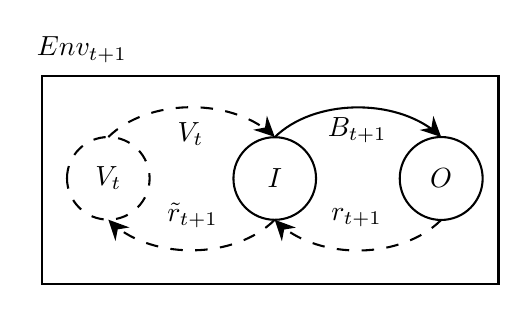
\begin{tikzpicture}[x=0.75pt,y=0.75pt,yscale=-1,xscale=1]
        
        %Shape: Circle [id:dp8739177923629333] 
        \draw   (123.48,130.05) .. controls (123.48,119.06) and (132.39,110.15) .. (143.38,110.15) .. controls (154.37,110.15) and (163.28,119.06) .. (163.28,130.05) .. controls (163.28,141.04) and (154.37,149.95) .. (143.38,149.95) .. controls (132.39,149.95) and (123.48,141.04) .. (123.48,130.05) -- cycle ;
        %Curve Lines [id:da2726669379173874] 
        \draw    (143.38,110.15) .. controls (161.99,91.83) and (200.82,90.88) .. (221.41,108.12) ;
        \draw [shift={(223.57,110.07)}, rotate = 224.02] [fill={rgb, 255:red, 0; green, 0; blue, 0 }  ][line width=0.08]  [draw opacity=0] (9.82,-4.72) -- (0,0) -- (9.82,4.72) -- (6.52,0) -- cycle    ;
        %Curve Lines [id:da4485667818478689] 
        \draw  [dash pattern={on 4.5pt off 4.5pt}]  (223.57,150.02) .. controls (204.36,169.14) and (165.2,169.5) .. (145.45,151.93) ;
        \draw [shift={(143.38,149.95)}, rotate = 405.89] [fill={rgb, 255:red, 0; green, 0; blue, 0 }  ][line width=0.08]  [draw opacity=0] (9.82,-4.72) -- (0,0) -- (9.82,4.72) -- (6.52,0) -- cycle    ;
        %Shape: Circle [id:dp8060688469385651] 
        \draw   (203.6,130.05) .. controls (203.6,119.01) and (212.54,110.07) .. (223.57,110.07) .. controls (234.6,110.07) and (243.55,119.01) .. (243.55,130.05) .. controls (243.55,141.08) and (234.6,150.02) .. (223.57,150.02) .. controls (212.54,150.02) and (203.6,141.08) .. (203.6,130.05) -- cycle ;
        %Shape: Rectangle [id:dp6054697635081123] 
        \draw   (31.2,80.5) -- (251.2,80.5) -- (251.2,180.83) -- (31.2,180.83) -- cycle ;
        %Shape: Circle [id:dp6091430023771998] 
        \draw  [dash pattern={on 4.5pt off 4.5pt}] (43.29,129.97) .. controls (43.29,118.98) and (52.2,110.07) .. (63.19,110.07) .. controls (74.18,110.07) and (83.09,118.98) .. (83.09,129.97) .. controls (83.09,140.96) and (74.18,149.87) .. (63.19,149.87) .. controls (52.2,149.87) and (43.29,140.96) .. (43.29,129.97) -- cycle ;
        %Curve Lines [id:da9876749075069771] 
        \draw  [dash pattern={on 4.5pt off 4.5pt}]  (143.38,149.95) .. controls (124.17,169.06) and (85.01,169.42) .. (65.26,151.85) ;
        \draw [shift={(63.19,149.87)}, rotate = 405.89] [fill={rgb, 255:red, 0; green, 0; blue, 0 }  ][line width=0.08]  [draw opacity=0] (9.82,-4.72) -- (0,0) -- (9.82,4.72) -- (6.52,0) -- cycle    ;
        %Curve Lines [id:da9412329086480583] 
        \draw  [dash pattern={on 4.5pt off 4.5pt}]  (63.19,110.07) .. controls (81.8,91.76) and (120.63,90.8) .. (141.21,108.05) ;
        \draw [shift={(143.38,110)}, rotate = 224.02] [fill={rgb, 255:red, 0; green, 0; blue, 0 }  ][line width=0.08]  [draw opacity=0] (9.82,-4.72) -- (0,0) -- (9.82,4.72) -- (6.52,0) -- cycle    ;
        
        % Text Node
        \draw (143.38,130.05) node  [font=\normalsize]  {$I$};
        % Text Node
        \draw (223.57,130.05) node  [font=\normalsize]  {$O$};
        % Text Node
        \draw (183.14,106.95) node  [font=\normalsize]  {$B_{t+1}$};
        % Text Node
        \draw (182.81,148.81) node  [font=\normalsize]  {$r_{t+1}$};
        % Text Node
        \draw (50.45,68.01) node  [font=\normalsize,rotate=-0.16]  {$Env_{t+1}$};
        % Text Node
        \draw (63.19,129.97) node  [font=\normalsize]  {$V_{t}$};
        % Text Node
        \draw (103.81,147.81) node  [font=\normalsize]  {$\tilde{r}_{t+1}$};
        % Text Node
        \draw (102.81,108.81) node  [font=\normalsize]  {$V_{t}$};
        \end{tikzpicture}
    \end{adjustbox}
  \end{center}
\caption{\textbf{The process of incentive salience attribution}. Solid and dashed elements represent respectively observable (i.e. behavioural) and latent aspects of the process. The individual and the object that they interact with are indicated by $I$ and $O$. The strength of the interaction is represented by $B$. The salience that $I$ attributes to $O$ is expressed by $V$ while $r$ and $\tilde{r}$ are the experienced reward and its weighted version produced by the state of $I$. All the contextual factors influencing both the amount of $r$ perceived and the magnitude of $B$ produced are represented by $Env$. The dynamical natures of the process is expressed though the arbitrary temporal unit $t$.}
\label{fig: incs}
\end{figure}